% !TEX root = ../Thesis.tex




\chapter{Extended Background} \label{cha:extendBackground}



This chapter provides the background for the thesis. It first introduces ERP systems and SAP as a general enterprise data-processing environment, then presents the industry and Volvo CE case context, outlines broader challenges in SAP-based enterprise workflow implementations, and finally reviews related work relevant to transparency, traceability, and usability in enterprise analytics.


\section{ERP Systems, SAP, and Enterprise Workflows}

Enterprise resource planning (ERP) systems are widely used to integrate and manage core business processes across large organizations \cite{davenport1998,klaus2000}. Rather than treating finance, operations, procurement, manufacturing, logistics, and sales as isolated activities, ERP systems provide a shared environment in which data and processes can be coordinated across functional boundaries \cite{sap_erp_guide}. In that sense, ERP should be understood not only as a transactional business system, but also as an enterprise data-processing setting environment in which important reporting, planning, and calculation processes are executed.

Prior literature indicates that ERP-based environments can support activities beyond basic transaction processing. Integrated enterprise data may also be reused for reporting, planning, performance monitoring, and analytical routines in different organizational settings \cite{monk2012erp,fan2006equipmentdw}. In this thesis, this is taken as support for viewing complex business calculations in enterprise systems as part of a broader workflow context rather than only as an isolated practice in one company.

SAP is one of the most widely used ERP platforms in this broader landscape. Within SAP-based environments, workflow execution is often distributed across data-loading mechanisms, storage structures, transformation logic, reporting layers, and user-facing interfaces. This makes SAP relevant to the present thesis not because it is unique to Volvo CE, but because it represents a common type of enterprise environment in which complex data-processing workflows are embedded.

Within the SAP landscape, transactional processing and analytical processing are typically separated. Operational data is generated in ERP systems, while SAP Business Warehouse (BW) provides an analytical layer for reporting, modeling, and transformation \cite{sap_bw_guide}. SAP also supports structured data loading, multidimensional storage, sequential rule execution, and spreadsheet-based user interaction \cite{sap_bw_ip_overview,sap_analysis_office_guide}. These capabilities make SAP suitable for complex multi-step workflows, but they also contribute to technical complexity.

This complexity is also reflected in prior work. Research on SAP ERP process extraction describes the identification of relevant process structures and related tables as a significant challenge because SAP ERP contains a large amount of process and data complexity \cite{weber2022sap}. ERP usability studies further report difficulties related to navigation, task support, learnability, and presentation of outputs \cite{calisir2004erp,wong2016sap}. Together, these studies support treating transparency, traceability, and usability as relevant concerns in ERP-based enterprise data processing beyond one company-specific case.




\section{Construction Equipment Industry and Market Share Estimation}




% The construction equipment industry is a global, capital-intensive sector supporting infrastructure development, mining, and urbanization. Leading manufacturers include Volvo Construction Equipment (Volvo CE), Caterpillar, Komatsu, Hitachi Construction Machinery, and Liebherr, all operating across multiple regions with diverse product portfolios \cite{offhighway2024report,statista2024construction}. These manufacturers maintain global distribution networks and sell equipment across a large number of countries, reflecting the highly international nature of the industry \cite{volvo2024annual}.

% Construction equipment is typically organized into machine lines, which represent major categories of machinery based on functionality. Common machine lines include hydraulic excavators, wheel loaders, articulated haulers, rigid haulers, and road construction equipment. Within each machine line, products are further segmented into size classes, usually defined by operating weight ranges (e.g., <6 tons, 6–10 tons, >10 tons), reflecting different application scenarios and customer needs \cite{mordor2024construction}.

% From a market analysis perspective, the industry is structured along dimensions including country, machine line, size class, and brand. Market size and share are therefore calculated at a granular level, allowing companies to evaluate performance in specific segments.

% To support market analysis, companies integrate multiple data sources. Internal data consists of sales records from enterprise systems.Companies also participate in industry data exchange systems, where aggregated sales information is shared among manufacturers to estimate total market size, often coordinated by industry associations or specialized providers such as Off-Highway Research \cite{offhighway2024report,offhighway2018method}. External datasets from third-party providers, dealer networks, and national registration systems further complement these sources, improving market coverage where direct reporting is limited \cite{mordor2024construction,oxford2023equipment}. These datasets are standardized and integrated to ensure consistency across countries, machine lines, and brands.
This thesis is grounded in the case of Volvo Construction Equipment (Volvo CE), whose market-analysis work is situated in the construction equipment industry. Industry reports describe a market that spans multiple countries, product segments, and regional conditions \cite{cece2025,mordor2024construction}. Because manufacturers operate across these dimensions, market analysis often depends on combining inputs for total market size and market share across regions and product categories.





% Market share is a widely used indicator to evaluate a firm’s competitive position within a defined market. It is typically defined as the ratio between a company’s sales and the total market size within a given segment \cite{kotler2016marketing}. In practice, business units within companies estimate both the total market size and their own share in order to assess competitive dynamics, benchmark performance against competitors, and support strategic planning and decision-making \cite{porter2008competitive}.

% In the construction equipment industry, estimating total market size requires integrating information from multiple sources. A common approach is based on the aggregation of sales data from different manufacturers. Industry intelligence providers such as Off-Highway Research collect and consolidate equipment sales data across regions and product categories, using inputs from manufacturers, dealers, and regional experts to construct a comprehensive view of the market \cite{offhighway2024report,offhighway2018method}. In practice, some manufacturers contribute aggregated sales data to industry research providers or participate in data exchange mechanisms, enabling the construction of comprehensive market statistics \cite{offhighway2018method,mordor2024construction}.

% In addition to manufacturer-reported data, external datasets are often used to complement market coverage. These may include dealer-reported sales, equipment registration statistics, and country-level estimates obtained from third-party providers. Such data sources are particularly important in markets where direct reporting is incomplete or inconsistent.Furthermore, some market research approaches incorporate statistical estimation and modelling techniques. These methods combine historical data with primary and secondary research, and in some cases use macroeconomic indicators to support market estimation and forecasting \cite{mordor2024construction,oxford2023equipment}.

% Based on these practices, data used for market share estimation in the construction equipment industry can generally be categorized into three types: internal company data, industry-level exchange or aggregated data, and external datasets obtained from third-party sources. These different data sources are typically combined to construct a consistent representation of the total market across countries, equipment types, and brands.



% % \section{Market Share Calculation in SAP Systems}


% % At Volvo CE, market share estimation is implemented through a structured Total Market Calculation (TMC) framework that integrates multiple datasets to reconstruct the total market and derive Volvo CE's competitive position.
% % The framework is built on three main data categories: internal sales data (SAL), representing Volvo CE's actual sales volumes; statistical exchange data (CRP) aggregated into total market data (TMA), providing a baseline estimate of overall market size; and additional external datasets (OTH), such as PIN and DES files, extending market coverage. Since these sources differ in structure, they are first transformed into standardized templates before further processing.

% % To enable consistent transformation, the framework relies on predefined matrices and configuration tables, including the Source Matrix, Reporter List, Country Grouping, Brand Mapping, and Size Class structures, which define how data is classified, aggregated, and linked across dimensions.
% % The total market is constructed using a hybrid logic: statistical exchange data provides the initial market size estimate, but since not all brands participate in reporting, the framework incorporates Volvo CE's internal sales data and applies transformation rules to reconstruct a more complete market representation. The implementation of this framework can be understood as a sequence of structured transformation steps, as summarized in Table 2.1.

% % \begin{table}[h]
% % \centering
% % \caption{Step-wise Process of the Market Share Framework at Volvo CE}
% % \label{tab:tmc_process}
% % \begin{tabular}{cll}
% % \toprule
% % \textbf{Step} & \textbf{Phase} & \textbf{Description} \\
% % \midrule
% % 1 & Data Collection & Regional data is collected from CRP, OTH files, and internal sales systems \\
% % 2 & Data Standardization & Input datasets are transformed into standardized templates \\
% % 3 & Matrix Application & Configuration tables (Source Matrix, Reporter List, Brand Mapping) are applied \\
% % 4 & Total Market Construction & Total market (TMA) is constructed based on statistical exchange data \\
% % 5 & Internal Data Integration & Volvo CE sales data (SAL) is integrated into the dataset \\
% % 6 & Reporter Identification & Brands are classified as reporting or non-reporting \\
% % 7 & Estimation of Missing Data & Volumes for non-reporting brands are estimated using rules \\
% % 8 & Segmentation and Allocation & Data is distributed across country, machine line, and size class \\
% % 9 & Market Share Calculation & Market share is calculated as Volvo sales divided by total market \\
% % \bottomrule
% % \end{tabular}
% % \end{table}



% % A defining characteristic of the framework is its multi-dimensional structure, where market share is calculated across country, machine line, and size class. For non-reporting brands where detailed breakdowns are unavailable, volumes are distributed across size classes based on the observed structure of the total market.

% % Overall, the TMC framework can be understood as a rule-based data integration and transformation system that combines internal and external sources to approximate market conditions through predefined matrices and sequential calculation steps.




% Market share is a widely used indicator to evaluate a firm’s competitive position within a defined market. It is typically defined as the ratio between a company’s sales and the total market size within a given segment \cite{kotler2016marketing}. In practice, business units within companies estimate both the total market size and their own share in order to assess competitive dynamics, benchmark performance against competitors, and support strategic planning and decision-making \cite{porter2008competitive}.




% Given the global and highly competitive nature of the construction equipment industry, manufacturers must continuously assess their performance across regions, product segments, and competitors. In this context, understanding market share becomes essential, as it provides a standardized indicator for evaluating competitive position, benchmarking against competitors, and supporting strategic planning and decision-making \cite{porter2008competitive, kotler2016marketing}. 



% However, due to the fragmented nature of data sources and the lack of a unified reporting standard across the industry, there is no universally accepted methodology for calculating total market size and market share. As a result, companies must estimate the total market and their relative position by integrating multiple data sources and applying internal assumptions and transformation rules. Consequently, companies require reliable and structured methods to estimate both the total market size and their market share, which motivates the need for systematic market share estimation approaches discussed in the following section. 












% In the construction equipment industry, estimating total market size requires integrating information from multiple sources. A common approach is based on the aggregation of sales data from different manufacturers. Industry intelligence providers such as Off-Highway Research collect and consolidate equipment sales data across regions and product categories, using inputs from manufacturers, dealers, and regional experts to construct a comprehensive view of the market \cite{offhighway2024report, offhighway2018method}. In practice, some manufacturers contribute aggregated sales data to industry research providers or participate in data exchange mechanisms, enabling the construction of comprehensive market statistics \cite{offhighway2018method, mordor2024construction}.

% In addition to manufacturer-reported data, external datasets are often used to complement market coverage. These may include dealer-reported sales, equipment registration statistics, and country-level estimates obtained from third-party providers. Such data sources are particularly important in markets where direct reporting is incomplete or inconsistent.\cite{mordor2024construction, oxford2023equipment}.

% Based on these practices, data used for market share estimation in the construction equipment industry can generally be categorized into three types: internal company data, industry-level exchange or aggregated data, and external datasets obtained from third-party sources. These different data sources are typically combined to construct a consistent representation of the total market across countries, equipment types, and brands. However, the integration of such heterogeneous data sources also introduces several challenges for enterprise-level implementation.

% First, structural and semantic inconsistencies arise because different data sources often follow different classification standards, levels of granularity, and reporting logic. For example, equipment categories, size classes, and brand definitions may not be aligned across sources, requiring complex mapping and transformation rules to ensure comparability.

% Second, data completeness is often limited. Not all manufacturers participate in data exchange mechanisms, and external datasets may only provide partial market coverage in certain regions. As a result, companies must reconstruct the total market using a combination of reported data and estimation logic, which increases the complexity of the calculation process.

% Third, maintaining consistency across multiple analytical dimensions, such as country, machine line, brand, and time, is challenging when combining heterogeneous datasets. Ensuring that aggregated values remain coherent across different levels of analysis requires carefully designed data processing logic.

% Finally, when such calculation processes are implemented within enterprise systems, additional challenges related to transparency and traceability arise. The underlying calculation logic is often embedded within complex system workflows, making it difficult for business users to understand, validate, or debug intermediate results.

% These challenges highlight the need for structured data processing frameworks that can integrate heterogeneous data sources while ensuring consistency, transparency, and maintainability in market share estimation.


% \subsection{Market Share Estimation in the Construction Equipment Industry and Associated Challenges}

% Given the global and highly competitive nature of the construction equipment industry, manufacturers must continuously assess their performance across regions, product segments, and competitors. In this context, market share serves as an important indicator for evaluating competitive position, benchmarking performance, and supporting strategic planning and decision-making \cite{porter2008competitive, kotler2016marketing}. However, due to the fragmented nature of available data and the lack of a unified reporting standard across the industry, there is no universally standardized methodology for calculating total market size and market share. Instead, companies must estimate both the overall market and their relative position by integrating multiple data sources and applying internal assumptions, mappings, and transformation rules.

% In practice, market share estimation in the construction equipment industry relies on combining information from several sources. A common approach is based on aggregating sales data from different manufacturers. Industry intelligence providers such as Off-Highway Research collect and consolidate equipment sales data across regions and product categories, using inputs from manufacturers, dealers, and regional experts to construct a broader view of the market \cite{offhighway2024report, offhighway2018method}. In some cases, manufacturers also participate in industry data exchange mechanisms or contribute aggregated sales data to research providers, which supports the construction of broader market statistics \cite{offhighway2018method, mordor2024construction}.

% To complement such reporting, external datasets are often incorporated to improve market coverage. These may include dealer-reported sales, equipment registration statistics, and country-level estimates obtained from third-party providers, especially in markets where direct reporting is incomplete or inconsistent \cite{mordor2024construction, oxford2023equipment}. Based on these practices, the data used for market share estimation can generally be grouped into three categories: internal company data, industry-level exchange or aggregated data, and external third-party datasets. These sources are then combined to form a consistent representation of the total market across countries, equipment types, and brands.

% Although this multi-source approach improves market coverage, it also introduces several challenges for enterprise-level implementation:

% \begin{itemize}
%     \item \textbf{Heterogeneous data structures and definitions.} Different data sources often follow different classification standards, levels of granularity, and reporting logic. Equipment categories, size classes, and brand definitions may not align across datasets, which creates a need for mapping and transformation rules before the data can be meaningfully compared.

%     \item \textbf{Incomplete market coverage.} Not all manufacturers participate in data exchange mechanisms, and some external datasets only provide partial visibility in specific countries or market segments. As a result, companies must reconstruct the total market using a combination of reported values and estimation logic.

%     \item \textbf{Cross-dimensional consistency requirements.} Market share estimation must remain coherent across multiple analytical dimensions, such as country, machine line, brand, and time. Maintaining consistency across these dimensions requires carefully designed aggregation and validation logic.

%     % \item \textbf{Limited transparency in enterprise implementation.} When market share calculation is implemented within enterprise systems, the logic is often embedded in complex data processing workflows. This can make intermediate transformations difficult for business users to understand, validate, or debug.
% \end{itemize}

% These challenges highlight the need for structured data processing frameworks that can integrate heterogeneous data sources while ensuring consistency, transparency, and maintainability in market share estimation.



In this industry setting, market share is a key indicator for assessing position and supporting strategic decision-making \cite{kotler2016marketing}. Yet market size and market share are rarely derived from one standardized source, so firms must combine internal sales data, industry-level exchange or aggregated data, and external third-party inputs.

In practice, market share estimation may involve combining internal company sales data, industry-level aggregated or exchange data, and external third-party datasets. Off-Highway Research describes the use of information from manufacturers, dealers, and regional sources in its market-estimation work \cite{offhighway2018method}. Industry reports also indicate that external sources can be used when reporting coverage is incomplete \cite{mordor2024construction}.

While this multi-source approach improves market coverage, it also introduces key challenges:

\begin{itemize}
    \item \textbf{Heterogeneous data structures:} Differences in classification standards, granularity, and definitions require data mapping and transformation before integration.

    \item \textbf{Incomplete coverage:} Not all market participants contribute data, requiring estimation and reconstruction of missing segments.

    \item \textbf{Cross-dimensional consistency:} Market share calculations must remain consistent across dimensions such as country, product category, brand, and time.
\end{itemize}

These challenges motivate structured data-processing frameworks that can integrate heterogeneous sources while keeping the workflow consistent, reliable, and understandable.



















% \section{Market Share Calculation in SAP Systems}

% % Enterprise resource planning (ERP) systems are widely used to manage and integrate business data across organizational functions, providing a foundation for analytical processes in industrial contexts \\cite{davenport1998,klaus2000}. Among these systems, SAP is one of the most widely adopted platforms, offering a centralized infrastructure for storing and managing large volumes of structured business data \cite{monk2012erp}.

% % Within SAP-based environments, analytical processes such as market share calculation are not implemented as single predefined functions, but rather as structured combinations of data integration, transformation, and aggregation. This reflects the broader characteristics of enterprise data processing, where analytical outcomes are derived through multi-step data pipelines rather than isolated functions \cite{vassiliadis2002etl}.

% % These processes follow data warehousing principles, where data from multiple operational systems must be integrated, cleaned, and harmonized before meaningful analysis can be performed \cite{inmon2005}. The integration of heterogeneous data sources introduces challenges related to structural differences and semantic inconsistencies, which must be resolved to ensure reliable analytical results \cite{lenzerini2002}.

% % SAP Business Warehouse (BW) provides the analytical layer that supports such processes. Its capabilities can be understood from two key perspectives.

% % \textbf{Data storage and multidimensional modeling.}\\
% % SAP BW organizes data using structured data models such as InfoCubes, where key figures are stored together with dimensions including product categories, geographical regions, and time periods. This multidimensional structure enables flexible aggregation and analysis across different perspectives, allowing key performance indicators to be calculated consistently. Such modeling approaches are consistent with dimensional data warehousing techniques designed for analytical processing \cite]{kimball2013}.

% % \textbf{Planning functions and processing sequences.}\\
% % In addition to data storage, SAP provides mechanisms for implementing calculation logic through planning functions and planning sequences. These mechanisms allow complex analytical processes to be decomposed into ordered sequences of transformations, ensuring that intermediate steps are applied in a controlled and reproducible manner. Similar stepwise execution models are commonly described in ETL and data processing workflows in enterprise systems \cite{vassiliadis2002etl}.

% % SAP systems provide a structured and scalable environment for supporting complex analytical processes. By combining integrated data storage, multidimensional modeling, and controlled processing logic, they enable the implementation of business calculations such as market share analysis. However, as discussed in the following section, this architecture also introduces challenges related to flexibility, transparency, and the integration of heterogeneous data sources.



% % 2.3 Market Share Calculation in SAP Systems

% % As Davenport \cite{davenport1998} and Klaus et al. \cite{davenport1998,klaus2000} point out, enterprise resource planning (ERP) systems are designed to integrate core business processes and consolidate operational data across organizational functions. Among these systems, SAP is one of the most widely adopted enterprise platforms, supporting business operations while also providing real-time data visibility and analytical capabilities \cite{sap_erp_guide}. 

% % In this sense, SAP should not be understood merely as a transactional system, but as a broader enterprise environment in which operational data can be loaded, structured, transformed, and reused for analytical purposes.



















% Within the broader SAP landscape, analytical processing is typically separated from transactional business processing. ERP systems generate and consolidate operational data, whereas SAP Business Warehouse (BW) structures and provides this data for analytical use, including reporting, modeling, and transformation \cite{sap_bw4hana_guide}. BW can therefore be understood as the analytical layer of the SAP ecosystem, on top of which more complex workflows, such as market share calculation, can be implemented.

% % As Vassiliadis et al. \cite{vassiliadis2002etl} argue, complex analytical results are generally produced through multi-step transformation workflows rather than isolated functions. Market share calculation in SAP can therefore be understood as one such workflow, implemented on top of SAP’s analytical infrastructure.

% From a technical perspective, SAP provides several components relevant to this type of calculation, including data input and loading mechanisms, analytical storage objects, multidimensional modeling structures, processing logic, and reporting outputs \cite{sap_analysis_office_guide,sap_bw_ip_overview}. Data enters the system through controlled upload and loading mechanisms, is stored in analytical structures such as InfoProviders, and is then processed through planning logic before being exposed to reporting layers.

% For market share calculation, SAP mainly provides two especially important capabilities:\\

%    \textbf {Data storage and multidimensional modeling}\\
% % SAP documentation on the enhanced star schema explains that an InfoCube stores key figures in a fact table, while characteristics are organized in surrounding dimensions \cite{sap_enhanced_star_schema}. SAP documentation on BW Integrated Planning further notes that aggregation levels define the subset of characteristics and key figures on which planning data can be entered, changed, and processed \cite{sap_bw_ip_overview}. This means that analytical data is structured according to business-relevant dimensions rather than treated as flat records only. For market share calculation, this is essential because key figures such as sales volume, market volume, and market share must be analysed consistently across country, machine line, brand, size class, and time. As Kimball and Ross \cite{kimball2013} point out, dimensional modeling provides the analytical basis for such aggregation and comparison across business perspectives.



% SAP BW supports market share calculation by organizing analytical data in a multidimensional structure rather than as flat records. In the classical BW model, an InfoCube is arranged according to SAP’s enhanced star schema, in which a central fact table stores key figures, while surrounding dimension tables store characteristics. The fact table contains only key figures, whereas the characteristics are kept in the dimensions, making it possible to analyze the same measures across multiple business perspectives.\cite{sap_enhanced_star_schema} For market share calculation, this is especially important because key figures such as sales volume, market volume, and market share must be consistently structured across dimensions such as country, machine line, brand, size class, and time. In this way, the enhanced star schema provides the technical storage model that enables multidimensional aggregation and comparison in SAP BW. \\


%   \textbf { Planning functions and processing sequences}\\

% SAP states that planning functions allow “system-based processing or generation of data,” while planning sequences group multiple planning functions and execute them sequentially \cite{sap_bw_ip_overview,sap_planning_sequences}. Technically, this provides an execution layer on top of the multidimensional data model. Rather than calculating market share in a single static query, SAP enables the process to be broken down into ordered operations such as copying, recalculation, deletion, distribution, and formula-based transformation \cite{sap_bw_ip_overview,sap_planning_functions}. SAP’s Analysis for Office documentation also shows that these planning objects can be triggered through Excel-based planning front ends, where users work with input-ready analytical data and execute planning logic from a spreadsheet interface \cite{sap_analysis_office_guide}. This is particularly relevant for market share calculation, since such calculations typically require several dependent steps, including data preparation, reconciliation, redistribution, and final aggregation.

% % Taken together, these capabilities explain why SAP can support complex market share calculation workflows. The multidimensional storage model provides a structured analytical basis on which heterogeneous market-related data can be aligned and compared, while the planning layer provides a controlled rule-based mechanism for transforming that data st

















% \section{Architecture of the Existing TMC Framework}
% \label{subsec:tmc_architecture}

% The current Total Market Calculation (TMC) framework at Volvo CE is implemented within an SAP Business Warehouse (BW) environment. It operates as a staged framework in which multiple data sources are loaded, transformed through rule-based processing steps, and subsequently transferred to a reporting layer. SAP therefore functions both as a storage environment and as the execution environment for market-share-related business logic.

% The framework combines source data, configuration matrices, and calculation logic into an integrated process. Source data is first loaded, after which predefined rules are applied to classify, reconcile, redistribute, and aggregate records across dimensions such as country, machine line, brand, and size class. Intermediate results are generated step by step before final outputs are prepared for reporting.

% \begin{figure}[htbp]
%     \centering
%     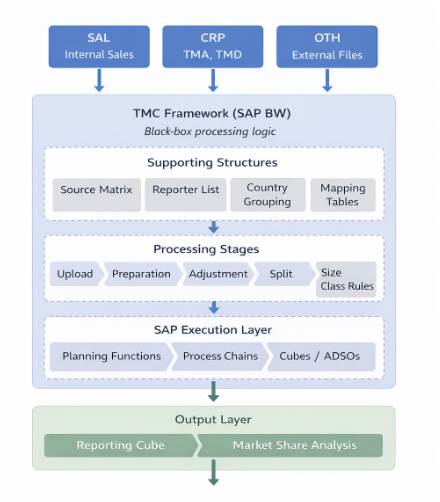
\includegraphics[width=0.9\textwidth]{tmc_architecture.png}
%     \caption{Overview of the SAP-based TMC framework and its main components.}
%     \label{fig:tmc_overview_architecture}
% \end{figure}




% \subsection{Data Sources and Supporting Structures}
% \label{subsec:tmc_data_sources}

% The TMC framework relies on three main categories of input data:

% \begin{itemize}
%     \item \textbf{SAL}: Volvo CE's internal sales data, serving as the authoritative source for its own sales volumes.
%     \item \textbf{CRP}: Statistical exchange data from the industry reporting environment, where \textit{TMA} provides the baseline estimate of the total market.
%     \item \textbf{OTH}: Externally uploaded data used to extend market coverage in cases where CRP reporting is incomplete.
% \end{itemize}

% To ensure comparability across these heterogeneous datasets, the framework depends on several supporting structures:

% \begin{itemize}
%     \item \textbf{Country grouping matrix}, used for aggregating data across geographical regions.
%     \item \textbf{Source matrix}, defining primary and secondary data sources for each market segment.
%     \item \textbf{Mapping tables}, standardizing brand and machine line classifications.
%     \item \textbf{Reporter list}, identifying which brands are treated as reporting entities.
%     \item \textbf{Size-class configuration rules}, ensuring consistency in size-based data processing and validation.
% \end{itemize}


% These supporting structures govern how records are interpreted and processed within the TMC workflow. In particular, the source matrix determines whether records proceed to subsequent calculation stages, while the reporter list influences whether records follow split-related logic or alternative processing paths.





% \subsection{Calculation Logic and SAP Execution} \label{subsec:tmc_calculation_logic} The TMC calculation follows a structured sequence of steps executed in SAP BW through Analysis for Office workbooks, upload interfaces, process chains, planning functions, and planning cubes. External file data is first uploaded and cleaned, CRP-based data is loaded through dedicated SAP processes, and the main TMC calculation is then executed on planning cubes. Final outputs are subsequently transferred to a reporting cube. The main calculation logic can be summarized as follows:

% \begin{itemize} \item \textbf{OTH upload and preprocessing:} External data is uploaded through an Analysis for Office workbook. The system validates the input structure, checks master data, and updates brand and machine-line mappings when necessary. The uploaded data is stored in an interface layer before being loaded into the analytical environment. \item \textbf{CRP upload:} CRP-based inputs, including TMA and SAL, are loaded through dedicated upload processes and consolidated into the TMC calculation environment.

% \item \textbf{Preparation -- CRP processing:} CRP data is processed first. Source-related flags, reporter distinctions, and intermediate reference values are derived. Volvo-related and non-Volvo market values are established here and reused in later split and restatement logic.

% \item \textbf{Preparation -- OTH processing:} OTH data is processed after CRP, since it depends on the reference values derived earlier. Source logic and reporter status are applied, and Volvo-related OTH records are excluded, as internal sales data is the authoritative source for Volvo CE's own volumes. 

% \item \textbf{Non-VCE total market calculation:} The non-VCE total market is derived as the difference between the overall market baseline and the Volvo-related portion, and is subsequently used as a proportional reference in later steps. 

% \item \textbf{Adjustment:} An adjustment value is calculated to keep the sum of FID values aligned with the total market baseline. Simultaneously, Volvo-related values from external market detail data are replaced by the corresponding internal sales values. This step acts both as a balancing mechanism and as a source-priority correction. 

% \item \textbf{Split:} Certain OTH records are available only in aggregated size-class structures that do not match the internal classification. These values are redistributed into finer segments using non-VCE total market values as the proportional reference, applied hierarchically from country to region to country-group level.

% \item \textbf{Total market construction:} All relevant records are consolidated, duplicate brand occurrences are removed, Volvo-related values are aligned with internal sales data, and the final total market is calculated by summing the remaining valid FID values. 

% \item \textbf{Restatement and reporting:} Selected values are recalculated proportionally to remain aligned with the reconstructed total market. The resulting dataset is transferred to the reporting layer for final market share analysis. \end{itemize}













% \begin{figure}
%     \centering
%     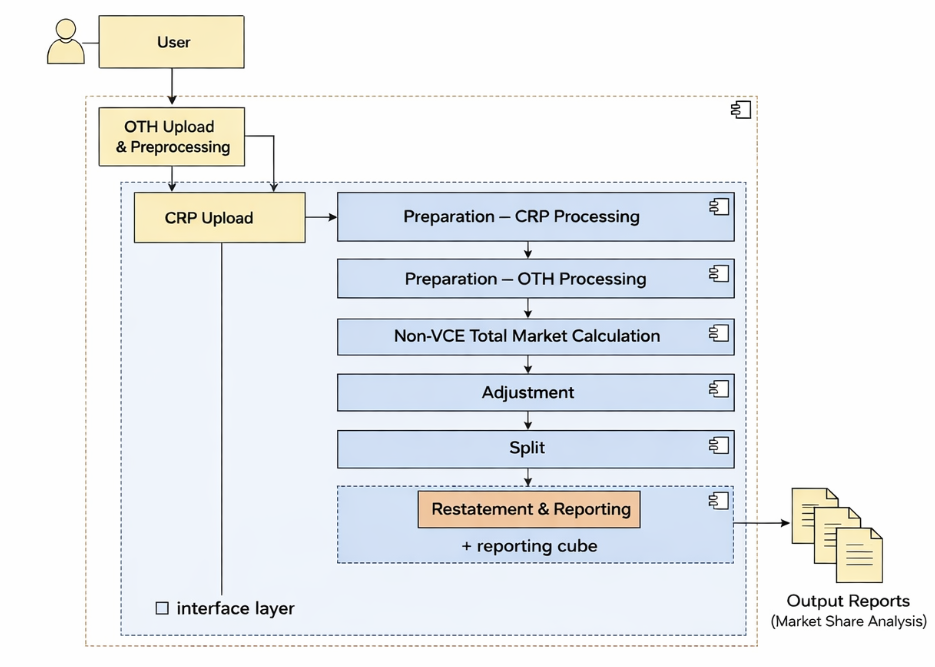
\includegraphics[width=0.9\linewidth]{tmc.png}
%     \caption{Execution flow of the SAP-based TMC framework from data upload to reporting}
%     \label{fig:tmc}
% \end{figure}







% The split step is particularly important because some external inputs are reported only in broader categories and must be translated into the finer classification required by the TMC framework. This redistribution uses the non-VCE total market structure as reference and is followed by a re-split validation step, in which implausible brand--size-class combinations are removed and remaining values are reallocated. This logic applies to reporter brands; non-reporters must already be uploaded in an appropriate size-class structure.

% For example, if an OTH record for a reporter brand is only available in the aggregated category $\text{CEX}_{\text{<10T}}$, the framework redistributes this value into $\text{CEX}_{\text{<6T}}$ and $\text{CEX}_{\text{6<10T}}$ using the non-VCE total market structure as reference. If a resulting brand--size-class combination is invalid according to the size-class configuration, it is removed and the remaining value is reallocated during the re-split step.

% Examples of typical split rules are shown below:

% \[
% \text{CEX}_{\text{<10T}} \rightarrow \{\text{CEX}_{\text{<6T}}, \text{CEX}_{\text{6<10T}}\}
% \]
% \[
% \text{GEC}_{\text{>6T}} \rightarrow \{\text{GEC}_{\text{6<10T}}, \text{GEC}_{\text{>10T}}\}
% \]
% \[
% \text{GEW}_{\text{>6T}} \rightarrow \{\text{GEW}_{\text{6<11T}}, \text{GEW}_{\text{>11T}}\}
% \]

% % \[
% % \text{WLO}_{\text{<10}} \rightarrow \{\text{WLO}_{\text{<7}}, \text{WLO}_{\text{7<10}}\}
% % \]



% \begin{figure}
%     \centering
%     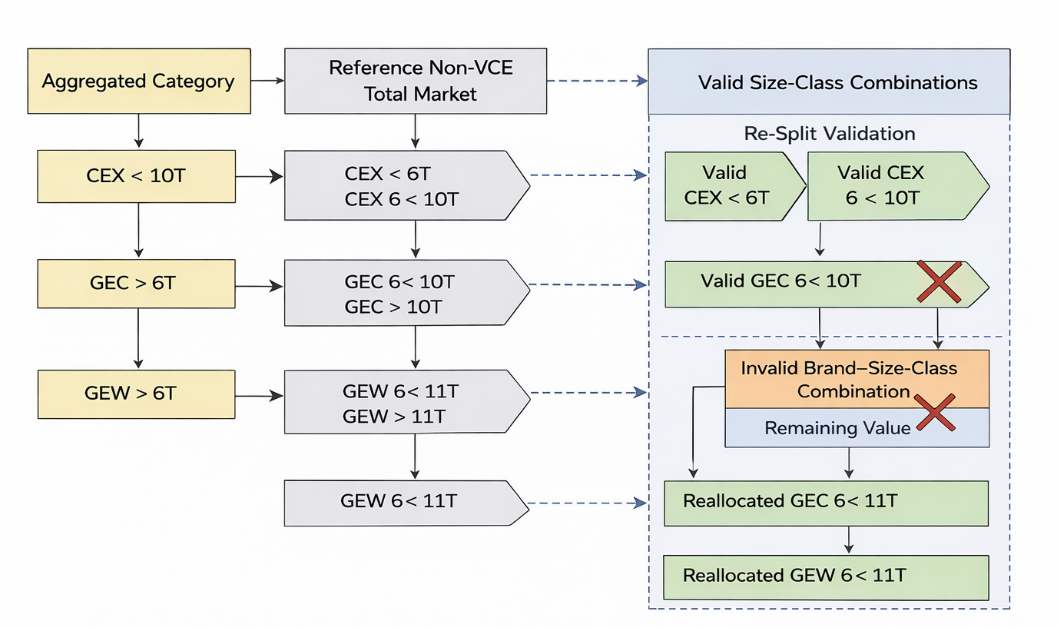
\includegraphics[width=0.9\linewidth]{split.png}
%     \caption{Illustration of split and re-split logic for aggregated OTH size-class categories.}
%     \label{fig:split}
% \end{figure}









% Overall, the SAP-based TMC framework can be understood as a layered reconstruction process in which source precedence, reporter classification, balancing adjustments, proportional redistribution, and controlled aggregation contribute to the final market share output. While analytically powerful, much of the logic is embedded inside SAP execution flows, making intermediate transformations less transparent to business users.










% 4.6.2026
% \section{Enterprise Implementation of Market Share Estimation at Volvo CE}
% \label{subsec:enterprise_tmc_volvo}

% To address the challenges of integrating heterogeneous market-related data and producing a consistent estimate of total market size, large manufacturers often implement dedicated calculation frameworks within enterprise systems. At Volvo CE, this is realized through a Total Market Calculation (TMC) framework implemented in an SAP-based analytical environment. The framework integrates multiple data sources, applies rule-based transformations, and generates the outputs used for market reporting and market share analysis.

% \subsection{ERP Systems and SAP as the Analytical Environment}

% Enterprise resource planning (ERP) systems are widely used to manage and integrate business data across organizational functions, thereby providing a foundation for analytical processes in industrial contexts \\cite{davenport1998,klaus2000}. Rather than treating business data as isolated records in separate applications, ERP systems consolidate operational information into a shared enterprise environment, making it possible to coordinate processes and reuse data across multiple business functions.

% Within the broader SAP landscape, analytical processing is typically separated from transactional business processing. ERP systems generate and consolidate operational data, whereas SAP Business Warehouse (BW) structures and provides this data for analytical use, including reporting, modeling, and transformation \cite{sap_bw4hana_guide}. BW can therefore be understood as the analytical layer of the SAP ecosystem, on top of which more complex workflows, such as market share calculation, can be implemented.

% From a technical perspective, SAP provides several components relevant to this type of calculation, including data input and loading mechanisms, analytical storage objects, multidimensional modeling structures, processing logic, and reporting outputs \cite{sap_analysis_office_guide, sap_bw_ip_overview}. Data enters the system through controlled upload and loading mechanisms, is stored in analytical structures such as InfoProviders, and is then processed through planning logic before being exposed to reporting layers.

% Two capabilities are particularly important for market share calculation. First, SAP BW organizes analytical data in a multidimensional structure rather than as flat records. In the classical BW model, an InfoCube follows SAP's enhanced star schema, in which a central fact table stores key figures and surrounding dimension tables store characteristics \cite{sap_enhanced_star_schema}. This makes it possible to analyze the same measures across multiple business perspectives. For market share calculation, this is essential because key figures such as sales volume, market volume, and market share must be structured consistently across dimensions such as country, machine line, brand, size class, and time.

% Second, SAP provides an execution layer through planning functions and planning sequences. SAP states that planning functions allow system-based processing or generation of data, while planning sequences group multiple planning functions and execute them sequentially \cite{sap_bw_ip_overview, sap_planning_sequences}. Rather than calculating market share in a single static query, SAP makes it possible to break the process into ordered operations such as copying, recalculation, deletion, distribution, and formula-based transformation \cite{sap_bw_ip_overview, sap_planning_functions}. In addition, SAP Analysis for Office enables such planning objects to be triggered through Excel-based planning front ends, where users work with input-ready analytical data and execute planning logic from a spreadsheet interface \cite{sap_analysis_office_guide}.

% Together, these capabilities provide the technical basis for implementing market share calculation in a structured and scalable enterprise environment. At Volvo CE, they support the TMC framework used to reconstruct the total market from multiple heterogeneous data sources.


\section{Enterprise Implementation of Market Share Estimation at Volvo CE}
\label{subsec:enterprise_tmc_volvo}

To understand how this broader problem appears in a real organizational setting, this thesis uses Volvo CE as a case study. Because market share estimation involves integrating heterogeneous data and applying repeatable rules across multiple business dimensions, firms may choose to implement such workflows in enterprise systems rather than rely only on isolated spreadsheets or ad hoc scripts. In the Volvo CE case, this is realized through a Total Market Calculation (TMC) framework implemented in SAP for market reporting and market share analysis.

\subsection{SAP as the Analytical Environment in the Volvo CE Case}

% Within the SAP landscape, analytical processing is typically separated from transactional business processing. ERP systems generate and consolidate operational data, whereas SAP Business Warehouse (BW) structures and provides this data for analytical use, including reporting, modeling, and transformation \cite{sap_bw4hana_guide}. BW can therefore be understood as the analytical layer of the SAP ecosystem, on top of which more complex workflows, such as market share calculation, can be implemented.

% From a technical perspective, SAP provides several components relevant to this type of calculation, including data input and loading mechanisms, analytical storage objects, multidimensional modeling structures, processing logic, and reporting outputs \cite{sap_analysis_office_guide, sap_bw_ip_overview}. Data enters the system through controlled upload and loading mechanisms, is stored in analytical structures such as InfoProviders, and is then processed through planning logic before being exposed to reporting layers.

% Two capabilities are particularly important for market share calculation. First, SAP BW organizes analytical data in a multidimensional structure rather than as flat records. In the classical BW model, an InfoCube follows SAP's enhanced star schema, in which a central fact table stores key figures and surrounding dimension tables store characteristics \cite{sap_enhanced_star_schema}. This makes it possible to analyze the same measures across multiple business perspectives. For market share calculation, this is especially important because key figures such as sales volume, market volume, and market share must be structured consistently across dimensions such as country, machine line, brand, size class, and time.

% Second, SAP provides an execution layer through planning functions and planning sequences. SAP states that planning functions allow system-based processing or generation of data, while planning sequences group multiple planning functions and execute them sequentially \cite{sap_bw_ip_overview, sap_planning_sequences}. Rather than calculating market share in a single static query, SAP makes it possible to break the process into ordered operations such as copying, recalculation, deletion, distribution, and formula-based transformation \cite{sap_bw_ip_overview, sap_planning_functions}. In addition, SAP Analysis for Office enables such planning objects to be triggered through Excel-based planning front ends, where users work with input-ready analytical data and execute planning logic from a spreadsheet interface \cite{sap_analysis_office_guide}.

% Together, these capabilities provide the technical basis for implementing market share calculation in a structured and scalable enterprise environment. In the case of Volvo CE, they support the TMC framework as a controlled enterprise data-processing setting for market-related data integration and calculation.


% Within the SAP landscape, analytical processing is typically separated from transactional business processing. ERP systems generate and consolidate operational data, while SAP Business Warehouse (BW) serves as the analytical layer for reporting, modeling, and data transformation \cite{sap_bw4hana_guide}. This separation enables enterprise-level analytical workflows to be implemented on top of integrated operational data.

% From a technical perspective, the implementation of market-related calculations in SAP relies on several key components:

% \begin{itemize}
%     \item \textbf{Data integration and storage:} Data is loaded through controlled upload interfaces and process chains, and stored in BW structures such as InfoProviders and planning cubes. These structures support multidimensional modeling based on SAP’s enhanced star schema, enabling consistent analysis across dimensions such as country, machine line, brand, and time \cite{sap_enhanced_star_schema}.

%     \item \textbf{Calculation and execution logic:} Business logic is implemented through planning functions and planning sequences, which execute ordered transformations such as copying, filtering, recalculation, and distribution \cite{sap_bw_ip_overview, sap_planning_sequences}. In practice, these operations are configured within SAP BW Integrated Planning and may involve underlying ABAP-based execution logic for system-level processing.

%     \item \textbf{User interaction and input:} Analysis for Office provides a spreadsheet-based front end through which users can input data, trigger planning sequences, and interact with analytical datasets \cite{sap_analysis_office_guide}.
% \end{itemize}

% Together, these components form a layered architecture in which SAP supports data integration, multidimensional storage, and rule-based execution within a unified enterprise environment. In the case of Volvo CE, this architecture provides the technical foundation for implementing the TMC framework as a structured analytical workflow.

% Within enterprise systems, analytical processing is typically separated from transactional operations. In the SAP landscape, operational data is generated and consolidated in ERP systems, while SAP Business Warehouse (BW) provides the analytical layer for reporting, modeling, and data transformation \cite{sap_bw4hana_guide}. This separation enables complex analytical workflows to be built on top of integrated enterprise data.

% From a technical perspective, SAP provides several core capabilities that support enterprise-level calculations such as market share estimation:

% \begin{itemize}
%     \item \textbf{Data integration and storage:} Data is loaded through structured upload mechanisms and process chains, and stored in BW objects such as InfoProviders and planning cubes. These structures follow a multidimensional model based on the enhanced star schema, enabling consistent analysis across dimensions such as country, product, and time \cite{sap_enhanced_star_schema}.

%     \item \textbf{Multidimensional modeling:} SAP BW organizes key figures and characteristics in a way that supports flexible aggregation and comparison across multiple business perspectives, which is essential for consistent market-related analysis.

%     \item \textbf{Execution of calculation logic:} Business logic is implemented through planning functions and planning sequences, which allow ordered, rule-based transformations such as copying, filtering, recalculation, and distribution \cite{sap_bw_ip_overview, sap_planning_sequences}. These operations are executed within the SAP environment and can be supported by underlying ABAP-based processing logic.

%     \item \textbf{User interaction and data input:} Tools such as Analysis for Office provide spreadsheet-based interfaces for data input, parameter control, and triggering calculation processes \cite{sap_analysis_office_guide}.
% \end{itemize}

% Together, these capabilities form a layered analytical environment in which data integration, storage, and rule-based processing are tightly coupled. This provides the technical foundation for implementing structured enterprise data-processing settings.



In the Volvo CE setting, SAP provides the technical environment in which the TMC process is carried out. Operational data is generated in enterprise systems, while SAP Business Warehouse (BW) provides the analytical layer for reporting, modeling, and transformation \cite{sap_bw_guide}. For this thesis, the key point is that SAP combines structured data loading, sequential rule execution, and spreadsheet-based user interaction \cite{sap_bw_ip_overview}. In the Volvo CE case, these capabilities form the technical foundation for a controlled enterprise data-processing setting, while also making the calculation logic difficult to inspect from a business-user perspective.












\subsection{The Existing TMC Process and Its SAP-based Implementation}
\label{subsec:tmc_process_implementation}

% At Volvo CE, market share estimation is implemented through an existing Total Market Calculation (TMC) framework within an SAP Business Warehouse (BW) environment. Rather than being executed as a single calculation, the framework operates as a staged analytical workflow in which supporting master data is first maintained, source data is then uploaded and processed, and final outputs are subsequently prepared for reporting.

% The framework combines several main categories of market-related data:

% \begin{itemize}
%     \item \textbf{SAL}: Volvo CE's internal sales data, representing the company's own recorded sales volumes.
%     \item \textbf{CRP}: Industry exchange data collected from the reporting environment and used as an important external input to the calculation process.
%     \item \textbf{TMA}: A market-level reference value derived from industry exchange data and used in later calculation stages.
%     \item \textbf{OTH}: Additional externally uploaded data used to complement market coverage where standard reporting is incomplete.
% \end{itemize}

% In addition to these source datasets, the framework depends on a dedicated master data maintenance layer. This layer includes supporting matrices and classification structures, such as brand-related information, country grouping, source definitions, participation settings, and size-class-related rules. These maintained structures provide the configuration basis on which subsequent uploads and calculations can be executed consistently.

% The framework combines several SAP components. Analysis for Office workbooks are used as spreadsheet-based front ends for maintaining master data and uploading external inputs. Dedicated upload processes and process chains manage the loading and movement of data across the SAP environment. The analytical data is then stored in SAP BW structures such as InfoProviders and planning cubes, where multidimensional characteristics and key figures can be processed consistently.

% The execution logic of the TMC framework is implemented through planning functions and planning sequences. These objects allow the system to perform ordered transformations on the analytical data, such as copying, filtering, recalculation, deletion, distribution, and formula-based processing. In this way, SAP provides not only the storage layer for market-related data but also the execution layer for rule-based calculation logic.

% Overall, the SAP-based TMC framework can be understood as a structured workflow consisting of master data maintenance, source data upload, staged calculation, validation, and reporting. Through this combination of configuration-driven processing and sequential execution logic, SAP enables Volvo CE to implement market share estimation in a controlled enterprise environment.




At Volvo CE, market share estimation is carried out through an SAP-based TMC implementation that combines maintained configuration data with several categories of workflow input, especially internal sales data (SAL), industry exchange data (CRP), derived total-market reference data (TMA), and supplementary external data (OTH). The process is staged rather than monolithic: master data and matrix rules are maintained first, source data is then loaded into BW structures, and calculation logic is executed through planning functions and planning sequences.

For the purposes of this thesis, three aspects of that implementation are most important. First, the process depends on maintained classification structures and mapping rules, not only on raw source files. Second, calculation is executed through sequential preparation, transformation, redistribution, and reporting stages. Third, the resulting logic is distributed across several SAP artefacts and interfaces rather than exposed as one inspectable process view. These characteristics make the Volvo CE TMC process a relevant case for studying transparency and traceability in ERP-based enterprise data processing.


\begin{figure}[H]
    \centering
    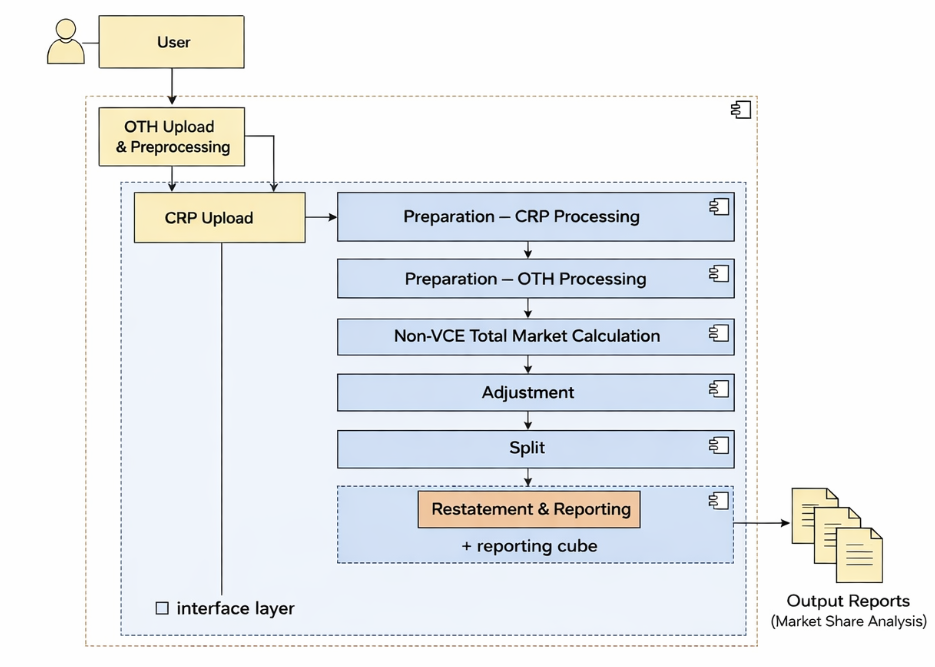
\includegraphics[width=0.9\linewidth]{tmc.png}
    \caption{Execution flow of the SAP-based TMC implementation from data upload to reporting.}
    \label{fig:tmc}
\end{figure}



\section{General Challenges in SAP-Based Enterprise Workflow Implementations}
\label{sec:sap_general_challenges}

The Volvo CE case is relevant because it reflects broader challenges that can arise when complex workflows are implemented in SAP-based enterprise environments. In such settings, business logic may be distributed across data-loading structures, maintained rules, planning objects, transformations, and reporting layers. Prior work on SAP ERP process identification highlights the difficulty of identifying relevant process structures and related tables in complex SAP environments \cite{weber2022sap}. ERP usability studies also report difficulties related to navigation, task support, presentation, and ease of use \cite{calisir2004erp,wong2016sap}.

Against that background, four general challenges are especially relevant to this thesis:

\begin{itemize}
    \item \textbf{Technical complexity:} Workflow logic may be implemented through SAP-specific objects such as planning functions, planning sequences, and other system-specific processing structures, which require specialized technical knowledge.

    \item \textbf{Limited transparency:} Processing may be executed across multiple system layers without one clear representation of the full workflow, making intermediate transformations difficult for business users to inspect and interpret.

    \item \textbf{Dependency on technical specialists:} When logic is embedded in system-specific structures, modifying, validating, or explaining workflow behavior may require technical support rather than direct business-user inspection.

    \item \textbf{Reduced traceability:} A distributed implementation can make it difficult to trace how data moves through transformations, verify intermediate results, and assess the effect of logic changes.
\end{itemize}

These broader challenges form the problem context for this thesis and are examined through the Volvo CE case study.








\section{Related Work}

To position these challenges in prior research, the literature relevant to this thesis can be grouped into three areas. First, data-warehouse and ETL literature describes enterprise analytics as staged workflows in which heterogeneous data is extracted, transformed, and prepared for reporting or decision support \cite{vassiliadis2009etl}. Related work on heterogeneous data integration shows that such workflows often involve inconsistent inputs and integration challenges \cite{putrama2024heterogeneous}. Work on data-pipeline quality similarly highlights transformation errors and related data-quality problems \cite{foidl2024pipeline}. This supports the need for explicit transformation stages and quality-control mechanisms in ERP-based enterprise data processing.

Second, ERP and SAP-related research highlights the complexity and usability challenges of enterprise systems. ERP systems integrate business processes across organisational functions \cite{klaus2000}. At the same time, that integration can introduce complex data structures, system-specific logic, and interfaces that require specialised knowledge \cite{davenport1998}. Research on SAP ERP process extraction shows that identifying relevant process structures and tables can be difficult in SAP environments \cite{weber2022sap}. ERP usability studies also show that navigation, task support, learnability, and output presentation affect end-user effectiveness \cite{calisir2004erp}. Similar concerns appear in SAP-related user settings \cite{wong2016sap}. These findings are relevant because the problem addressed in this thesis concerns not only workflow execution, but also whether business users can inspect and validate how outputs are produced.

Third, decision-support and enterprise analytics literature suggests that analytical functionality can be supported through additional user-facing layers that help users review data and interpret outputs \cite{march2007dss}. Work in the construction domain similarly shows that data-warehouse and decision-support layers can support analytical tasks beyond transactional enterprise systems \cite{fan2006equipmentdw}. Such layers can complement existing enterprise systems by providing more accessible interfaces for inspection, comparison, and validation.

Taken together, this literature supports the problem framing used in this thesis: ERP-based enterprise data processing can be technically robust and operationally useful while still being difficult for business users to inspect step by step. Within the literature reviewed for this thesis, no concrete browser-based design example was identified that re-expresses selected SAP-based workflow logic as explicit, reviewable stages for business users. This thesis addresses that gap through a Design Science Research study using Volvo CE's Total Market Calculation process as the empirical case study, while framing the underlying problem as a broader ERP-based enterprise data-processing challenge.
























